% Chapter 1

\chapter{Introducción general} % Main chapter title

\label{Chapter1} % For referencing the chapter elsewhere, use \ref{Chapter1} 
\label{IntroGeneral}

Este capítulo introduce el contexto del trabajo, expone los desafíos vinculados a la calidad del aire. Además, describe brevemente el sistema desarrollado, presenta los objetivos planteados y anticipa la estructura del documento.

%----------------------------------------------------------------------------------------

% Define some commands to keep the formatting separated from the content 
\newcommand{\keyword}[1]{\textbf{#1}}
\newcommand{\tabhead}[1]{\textbf{#1}}
\newcommand{\code}[1]{\texttt{#1}}
\newcommand{\file}[1]{\texttt{\bfseries#1}}
\newcommand{\option}[1]{\texttt{\itshape#1}}
\newcommand{\grados}{$^{\circ}$}

%----------------------------------------------------------------------------------------

%\section{Introducción}

%----------------------------------------------------------------------------------------
\section{Desafios ambientales}

La calidad del aire constituye un componente esencial para la salud pública y el bienestar colectivo. En las últimas décadas, el crecimiento acelerado de los entornos urbanos, junto al aumento de la actividad industrial y el incremento del parque automotor, provocó un deterioro progresivo en las condiciones atmosféricas de numerosas ciudades. 

Este fenómeno desató un incremento en la concentración de contaminantes como el material particulado (PM2.5 y PM10), el dióxido de nitrógeno (NO2), el dióxido de carbono (CO2) y diversos compuestos orgánicos volátiles (VOCs). Estos elementos impactan negativamente sobre la salud respiratoria, neurológica y cardiovascular de la población expuesta \cite{WHO:2021}.

Organismos como la Organización Mundial de la Salud (OMS) actualizaron en 2021 sus valores guía para la exposición a contaminantes atmosféricos \cite{WHO:2021}. La revisión incorporó nueva evidencia que demostró efectos adversos en la salud incluso en niveles inferiores a los considerados seguros anteriormente. Entre los grupos más vulnerables se encuentran niños, personas mayores y quienes presentan enfermedades respiratorias o cardiovasculares \cite{WHO:2018}. Este escenario exige a las autoridades de salud y medioambiente contar con herramientas confiables, accesibles y en tiempo real para monitorear la calidad del aire y fundamentar decisiones informadas.

Según el inventario de emisiones de gases de efecto invernadero de la Ciudad Autónoma de Buenos Aires \cite{GCBA:2022}, se alcanzaron un total de 11 189 391 toneladas de CO2 equivalente por año. Los principales emisores fueron el sector energético, con el 55 \% del total; el transporte, con un 28 \%; y el sector de residuos, que contribuyó con el 17 \% de las emisiones.

Ante este escenario, se identificó la necesidad de contar con herramientas tecnológicas que permitan monitorear la calidad del aire de manera distribuida, accesible y en tiempo real. Las soluciones basadas en Internet de las Cosas (IoT) ofrecen una alternativa viable para ampliar la cobertura de medición, reducir costos y facilitar el acceso a la información ambiental.

%----------------------------------------------------------------------------------------

\subsection{Descripción general del sistema}

El trabajo se centró en el desarrollo de un sistema de monitoreo de calidad de aire basado en tecnologías de Internet de las Cosas (IoT). Se abordó desde un enfoque tecnológico que integró microcontroladores, sensores ambientales, comunicación inalámbrica y una interfaz digital para visualizar datos.

Las mediciones se registran de manera periódica por los nodos sensores y se transmiten a una infraestructura central. El mecanismo de envío se define según el entorno operativo, en función de la disponibilidad de red y la distancia.

El sistema central recibe, valida y almacena los datos generados por cada nodo. Para asegurar la integridad del proceso, se emplean esquemas de autenticación y cifrado. Se cuenta con una aplicación web para las visualizaciones privadas y públicas según los privilegios del tipo de usuario.

Se contempló una arquitectura multiempresa, donde cada organización puede gestionar zonas, dispositivos y usuarios supervisores desde un panel administrativo. Se pretende utilizarlo como una herramienta de bajo costo, escalable y adaptable a distintos contextos urbanos e industriales.

\subsection{Introducción al índice de calidad del aire AQI}

El Índice de Calidad del Aire (AQI) desarrollado por la Agencia de Protección Ambiental de los Estados Unidos (EPA) \cite{EPA:2025}, se ha consolidado como un estándar internacional para comunicar niveles de contaminación atmosférica. La aplicación de la escala se ilustra en la figura \ref{fig:1_5-AQI}:

\begin{figure}[h]
    \centering
    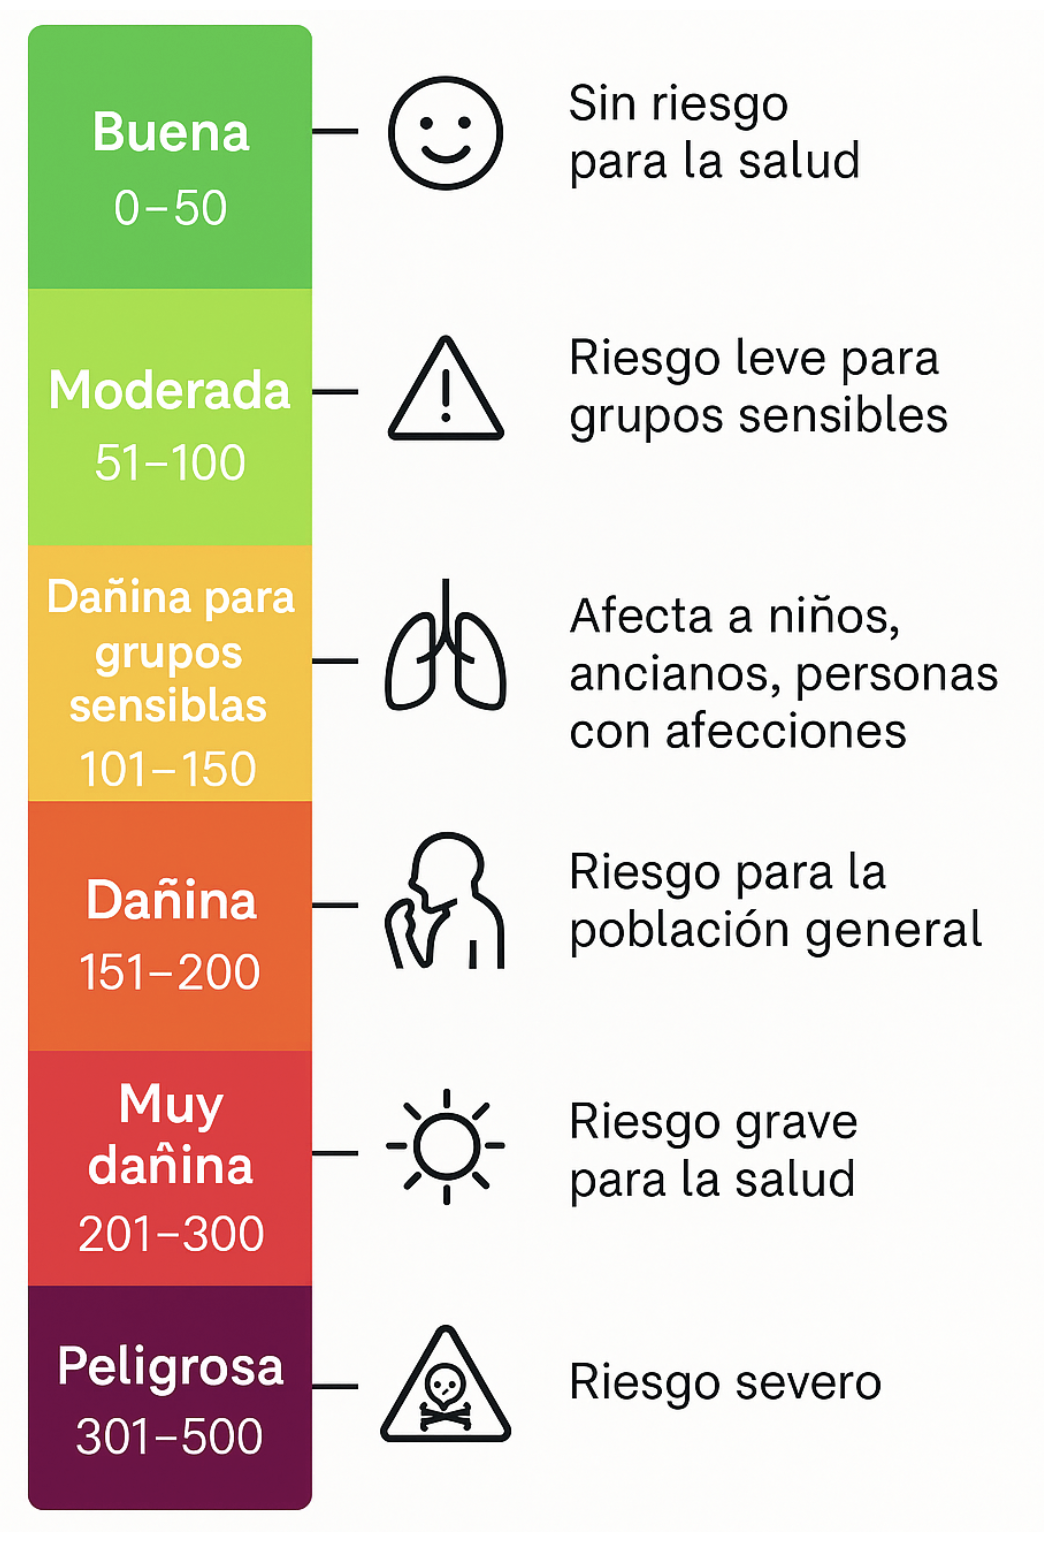
\includegraphics[width=0.45\linewidth]{Figures/1_5-AQI.png}
    \caption{Escala del Índice de Calidad del Aire (AQI)\protect\footnotemark.}
    \label{fig:1_5-AQI}
\end{figure}

\footnotetext{Fuente: Adaptado de \cite{EPA:2025} Guía mejorada sobre sensores de aire, Apéndice E.}

La escala abarca valores desde “buena” (0–50) hasta “peligrosa” (301 o más), con colores codificados que facilitan la interpretación pública y se acompañan de recomendaciones sanitarias específicas. Valores entre 101 y 150 indican un riesgo moderado para grupos sensibles, mientras que los superiores a 300 reflejan condiciones de riesgo severo para toda la población.

El AQI se emplea ampliamente para emitir alertas ambientales, orientar a la ciudadanía y respaldar la formulación de políticas públicas. En este trabajo, se adoptó su lógica estructural como referencia para las variables monitoreadas. Además, se prevé su futura incorporación como indicador compuesto dentro de la plataforma.

%----------------------------------------------------------------------------------------

\section{Motivación y propósito}

El presente trabajo surge ante la necesidad de contar con herramientas accesibles, confiables y adaptables para el monitoreo de la calidad del aire en contextos urbanos e industriales. En muchas ciudades de América Latina, las estaciones oficiales de medición resultan insuficientes para cubrir de forma representativa la diversidad de zonas expuestas a fuentes de contaminación.

Estas limitaciones responden, en parte, a los elevados costos de adquisición y mantenimiento de los equipos tradicionales. Además, los sistemas disponibles suelen operar de manera centralizada, con baja granularidad espacial y escasa participación de los actores locales en la recolección o consulta de datos ambientales.

En este escenario, el uso de tecnologías de IoT ofrece una oportunidad concreta para descentralizar la medición, reducir costos operativos y facilitar el acceso a información ambiental en tiempo real. La posibilidad de desplegar nodos sensores compactos, de bajo consumo y conectividad flexible, habilita nuevos modelos de monitoreo orientados a la acción local y al control preventivo.

El propósito de este trabajo fue diseñar e implementar una solución IoT integral, que permita capturar variables críticas de calidad del aire y presentar la información mediante una plataforma web de fácil acceso. La propuesta se enfocó en lograr una arquitectura modular, segura y escalable, capaz de adaptarse a distintos entornos y requerimientos institucionales o comunitarios.

%----------------------------------------------------------------------------------------

\section{Estado del arte}

El monitoreo de calidad del aire se ha abordado históricamente mediante estaciones fijas de alta precisión, operadas por organismos estatales o científicos. Estas estaciones, si bien confiables, requieren infraestructura costosa y tienen cobertura limitada \cite{EPA:2025}.

Frente a estas limitaciones, surgieron soluciones basadas en sensores de bajo costo. Estos dispositivos permiten ampliar la cobertura geográfica y acercar el monitoreo a zonas sin medición previa, aunque presentan desafíos en calibración y control de calidad \cite{Morawska:2018, Castell:2017}.

Plataformas internacionales como Sensor.Community, OpenAQ y PurpleAir promueven el monitoreo colaborativo mediante redes abiertas de sensores ciudadanos. Si bien lograron amplia capilaridad, en muchos casos carecen de trazabilidad, autenticación o validación técnica \cite{SensorCommunity:2025, OpenAQ:2020, PurpleAir:2021}.

A nivel comercial, empresas como IQAir y Clarity ofrecen soluciones avanzadas con visualización web, conectividad integrada y validación parcial, aunque a un costo elevado. En América Latina, se identificaron desarrollos universitarios y ciudadanos que implementan sensores económicos con visualización básica. Sin embargo, pocos integran funcionalidades como backend seguro, cifrado o control por roles \cite{Alvarez:2021, FIUBA:2023}.

En el trabajo desarrollado se combinan sistemas de bajo costo con características institucionales. Se integran sensores específicos, Wi-Fi, LoRaWAN, cifrado TLS, base de datos estruccturada, interfaz moderna y arquitectura multiusuario. Su diseño modular y replicable asegura flexibilidad y escalabilidad \cite{EPA:2025}.

La tabla \ref{tab:comparacion-soluciones} presenta una comparación entre soluciones actuales y el sistema desarrollado en este trabajo, con base en criterios técnicos y de implementación.

\begin{table}[h]
	\centering
	\caption[Comparación resumida de soluciones de monitoreo]{Comparación de soluciones de monitoreo ambiental según criterios técnicos y operativos.}
	\label{tab:comparacion-soluciones}
	\begin{tabular}{p{4cm} p{2cm} p{2cm} p{2.2cm}}   
		\toprule
		\textbf{Criterio} & \textbf{Estación tradicional} & \textbf{Sensor ciudadano (Luftdaten)} & \textbf{Propuesta desarrollada} \\
		\midrule
		Costo por nodo               & Muy alto   & Bajo         & Medio-bajo \\
		Precisión                    & Alta       & Media        & Media \\
		Cobertura geográfica         & Baja       & Alta         & Media-alta \\
		Comunicación segura (TLS)    & Sí         & No           & Sí \\
		Backend estructurado         & Sí         & No           & Sí \\
		Visualización en tiempo real & No siempre & Parcial      & Sí \\
		Gestión multiempresa         & No         & No           & Sí \\
		Escalabilidad                & Limitada   & Alta         & Alta \\
		\bottomrule
	\end{tabular}
        \footnotetext{Fuente: Adaptado de \cite{EPA:2025, Morawska:2018, Castell:2017, SensorCommunity:2025} y elaboración propia para la propuesta desarrollada.}
\end{table}

%----------------------------------------------------------------------------------------

\section{Objetivos y alcance}

Este trabajo desarrolla un sistema de monitoreo de calidad del aire orientado a contextos urbanos e industriales de América Latina. Utiliza tecnologías de Internet de las Cosas (IoT) para proporcionar una solución técnica viable, replicable y segura. Su diseño fomenta la descentralización de la recolección de datos ambientales y la democratización de su acceso.

El sistema presenta una arquitectura distribuida con nodos sensores, comunicación inalámbrica, un backend seguro y una plataforma web de visualización. Incorpora sensores de bajo costo, protocolos seguros de transmisión y una interfaz accesible, para usuarios con distintos niveles de experiencia.

El sistema fue concebido como una herramienta de apoyo para instituciones públicas, empresas y comunidades interesadas en conocer las condiciones ambientales en tiempo casi real. Ofrece utilidad para fines educativos, de investigación y de participación ciudadana. Su diseño promueve la toma de decisiones informadas en diversos contextos.

\subsection{Objetivo general}
Diseñar un sistema IoT para monitorear la calidad del aire en entornos urbanos e industriales, seguro, escalable y con disponibilidad de los datos de forma privada y pública.

\subsection{Objetivos específicos}
\begin{itemize}
    \item Construir nodos sensores basados en microcontroladores con conectividad Wi-Fi y LoRaWAN.
    \item Integrar sensores para la medición de material particulado, gases contaminantes, compuestos orgánicos volátiles, temperatura y humedad.
    \item Implementar un backend en Node.js con base de datos MongoDB y protocolos seguros de comunicación (MQTT con TLS).
    \item Desarrollar una interfaz web moderna para la visualización de datos en tiempo real, históricos y administración de usuarios.
    \item Validar el funcionamiento del sistema en condiciones reales y evaluar su escalabilidad técnica.
\end{itemize}

\subsection{Alcance y limitaciones}
El alcance del trabajo comprendió el desarrollo completo de una primera versión funcional del sistema, con nodos sensores, backend, base de datos y frontend. Se simuló el funcionamiento del sistema en entornos controlados, sin realizar campañas extensas de medición ambiental en campo.

No se abordaron tareas de calibración profesional de sensores ni validaciones frente a instrumentos de referencia. Tampoco se desarrollaron funcionalidades de análisis predictivo, detección de anomalías o clasificación automática.

La solución se orientó principalmente a contextos urbanos de pequeña o mediana escala, donde se disponga de conectividad mínima para la transmisión de datos. El despliegue en zonas rurales, en ausencia total de infraestructura de red, no formó parte del alcance de esta etapa.

%----------------------------------------------------------------------------------------